\section{Getting Started with \LaTeX}

{
\paper{
	\textbf{Cheng 2020} in \faGithub https://github.com/xu-cheng/latex-tutorial
	}

\begin{frame}{Introduction}
  \begin{itemize}
    \item \alert{\LaTeX{}} is a document preparation system and document markup language.
    \item It can be used to typeset articles, books, slides, posters, even graphics.
    \item \textbf{\textcolor{Green}{Pros}:}
          \begin{itemize}
            \item It separates presentation/format from contents.
            \item Since the source codes are plaintext, it works well with version control system such as git.
            \item Highly customizable through various of packages.
          \end{itemize}
    \item \textbf{\textcolor{Red}{Cons}:}
          \begin{itemize}
            \item There is no graphic interface to support WYSIWYG style editing.
            \item Not suitable to produce unstructured documents.
          \end{itemize}
  \end{itemize}
\end{frame}
}

\begin{frame}[fragile]{Installation}
  \begin{itemize}
    \item \textbf{Windows/Linux}
          \begin{itemize}
            \item TeXLive \url{https://www.tug.org/texlive/}
            \item Online installer:
                  \begin{itemize}
                    \item Windows \\ \url{http://mirror.ctan.org/systems/texlive/tlnet/install-tl-windows.exe}
                    \item Linux \\ \url{http://mirror.ctan.org/systems/texlive/tlnet/install-tl-unx.tar.gz}
                  \end{itemize}
            \item Offline ISO file:
                  \footnotesize
                  \url{http://mirror.ctan.org/systems/texlive/Images/}
          \end{itemize}
    \item \textbf{Mac}
          \begin{itemize}
            \item MacTeX \url{http://www.tug.org/mactex/}
            \item Or install through Homebrew (\url{https://brew.sh}) \\
                  \begin{minipage}{\linewidth+2.1em}
                    \inputminted[fontsize=\scriptsize]{bash}{./minted/install_mactex.sh}
                    \vspace{-2ex}
                  \end{minipage}
          \end{itemize}
    \item TeXLive/MacTeX release major updates around May each year. \\
          It is recommended to uninstall the old version and install the new version annually.
  \end{itemize}
\end{frame}


\begin{frame}{\LaTeX~editor}
  \begin{itemize}
    \item \LaTeX~source codes are plaintext. So you can use any editor you like.
    \item \textbf{Visual Studio Code \alert{[Recommend]}}
          \begin{itemize}
            \item \footnotesize \url{https://code.visualstudio.com}
            \item LaTeX Workshop \footnotesize \url{https://github.com/James-Yu/LaTeX-Workshop}
            \item Code Spell Checker \footnotesize \url{https://github.com/streetsidesoftware/vscode-spell-checker}
          \end{itemize}
    \item \textbf{Vim/Neovim}
          \begin{itemize}
            \item \footnotesize \url{https://www.vim.org} | \url{https://neovim.io}
            \item Vimtex \footnotesize \url{https://github.com/lervag/vimtex}
          \end{itemize}
    \item \textbf{Emacs}
          \begin{itemize}
            \item \footnotesize \url{https://www.gnu.org/s/emacs}
            \item AUCTeX \footnotesize \url{https://www.gnu.org/software/auctex}
          \end{itemize}
    \item \textbf{TeXstudio}
          \begin{itemize}
            \item \footnotesize \url{https://www.texstudio.org}
          \end{itemize}
  \end{itemize}
\end{frame}

\begin{frame}{Overleaf}
  \begin{itemize}
    \item \alert{Overleaf} (\url{https://www.overleaf.com/}) is a online, collaborative LaTeX editor
    \item Free for personal use
    \item \$15/month to share project among up to 10 collaborators
  \end{itemize}

  \begin{figure}
    \centering
    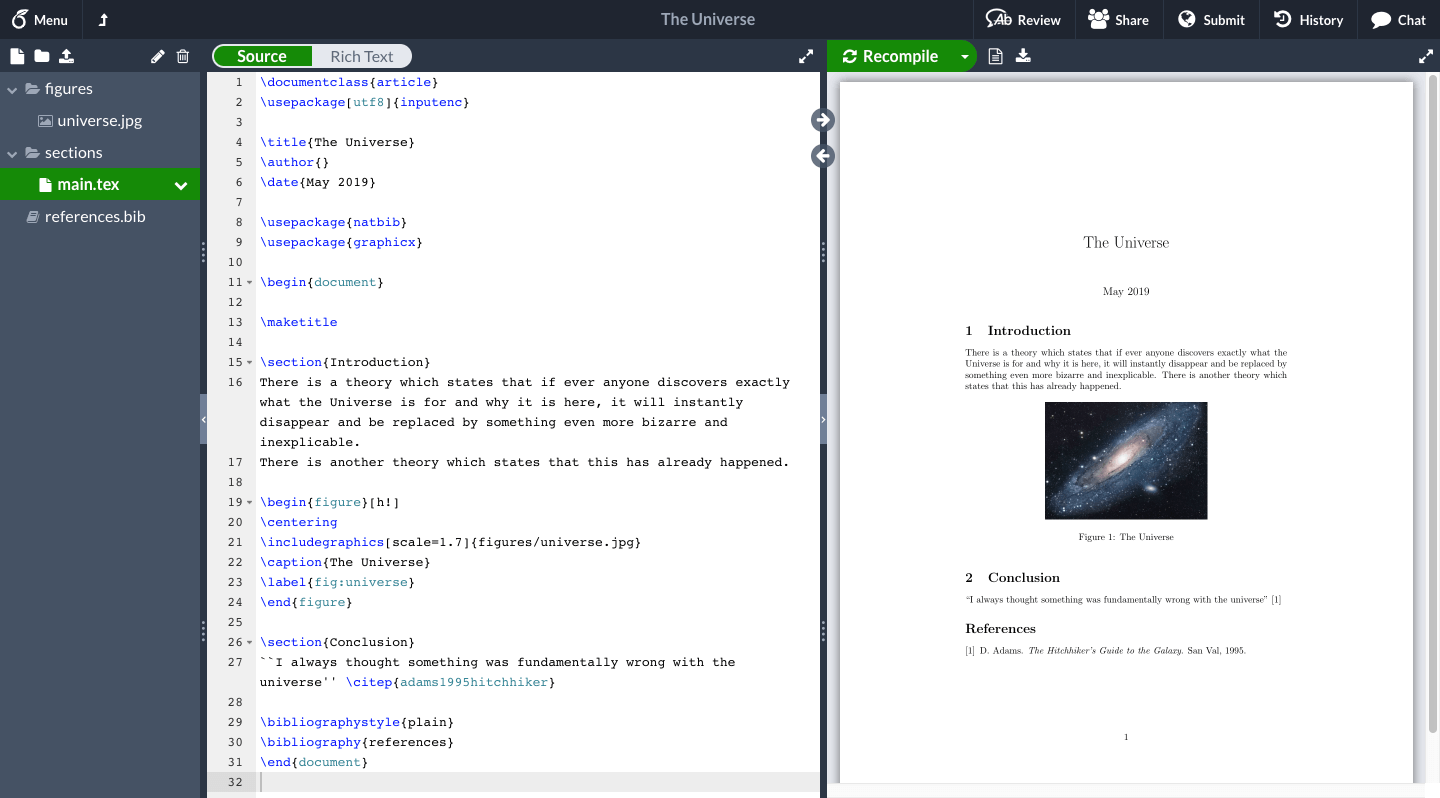
\includegraphics[width=.7\linewidth]{./figs/overleaf.png}
  \end{figure}
\end{frame}

